\documentclass{article}
\usepackage{graphicx}
\usepackage{float}  
\usepackage[utf8]{inputenc}
\usepackage[includeheadfoot, margin=1em,headheight=2em]{geometry}
\usepackage{titling}
\usepackage{hyperref}
\geometry{a4paper, left=2cm, right=2cm, top=2cm, bottom=2cm}
\usepackage{graphicx}
\providecommand{\versionnumber}{1.1.1}
\usepackage{enumitem}
\usepackage{array}
\newcolumntype{P}[1]{>{\centering\arraybackslash}p{#1}}
\renewcommand{\arraystretch}{1.5} % Default value: 1
\setlength{\droptitle}{-6em}
\usepackage{capt-of}
\usepackage{setspace}

%font
\usepackage[defaultfam,tabular,lining]{montserrat}
\usepackage[T1]{fontenc}
\renewcommand*\oldstylenums[1]{{\fontfamily{Montserrat-TOsF}\selectfont #1}}

%custom bold 
\usepackage[outline]{contour}
\usepackage{xcolor}
\newcommand{\custombold}{\contour{black}}

%table colors
\usepackage{color, colortbl}
\definecolor{Blue}{rgb}{0.51,0.68,0.79}
\definecolor{LightBlue}{rgb}{0.82,0.87,0.90}
\definecolor{LighterBlue}{rgb}{0.93,0.95,0.96}

\usepackage{caption}
\captionsetup[figure]{labelformat=empty}

%Header
\usepackage{fancyhdr, xcolor}
\pagestyle{fancy}
\let\oldheadrule\headrule% Copy \headrule into \oldheadrule
\renewcommand{\headrule}{\color{Blue}\oldheadrule}% Add colour to \headrule
\renewcommand{\headrulewidth}{0.2em}
\fancyhead[L]{Piano di qualifica}
\fancyhead[C]{Cybersorceres}
\fancyhead[R]{versione \versionnumber}

\title{\Huge{\textbf{Piano di Qualifica}}\vspace{-1em}}
\author{CyberSorcerers Team}
\date{}
\begin{document}
\maketitle
\vspace{-3em}
\begin{figure}[h]
  \centering
  
\includegraphics[width=6cm, height=6cm]{documenti/logo rotondo.png}
  \label{fig:immagine}
\end{figure}

\vspace{6em}
\large{
\begin{center}
    \begin{tabular}{P{24em}}
        \rowcolor{Blue}
        \textbf{Membri del team:}\\
        \rowcolor{LighterBlue}
        \custombold{Sabrina Caniato}\\
        \rowcolor{LightBlue}
        \custombold{Giulia Dentone}\\
        \rowcolor{LighterBlue}
        \custombold{Nicola Lazzarin}\\
        \rowcolor{LightBlue}
        \custombold{Giovanni Moretti}\\
        \rowcolor{LighterBlue}
        \custombold{Andrea Rezzi}\\
        \rowcolor{LightBlue}
        \custombold{Samuele Vignotto}\\
    \end{tabular}
\end{center}

\begin{center}
    \begin{tabular}{l c c}
        \rowcolor{Blue} 
        \textbf{Informazioni sul documento} & &\\ [1 ex]
        \rowcolor{LighterBlue}
        Destinatari: & Prof Tullio Vardanega & Prof Riccardo Cardin\\ [1 ex]
        \rowcolor{LightBlue}
        G al pedice: & Consultare il Glossario & \\ [1 ex]
    \end{tabular}
\end{center}
    
\newpage

\textbf{Registro dei Cambiamenti - Changelog\textsubscript{G}}
\begin{center}
\begin{tabular}{P{4em} P{6em} P{8em} P{8em} P{10em}} 
  \rowcolor{Blue}
    \custombold{Versione} & \custombold{Data} & \custombold{Autore} &
    \custombold{ Verificatore} & \custombold{Dettaglio}\\
    \rowcolor{LightBlue}
    1.1.1 & 06/05/2024 & Giulia Dentone & Samuele Vignotto & Corretta ed estesa la sezione di Valutazione per il miglioramento. \\ 
    \rowcolor{LighterBlue}
    1.1.0 & 04/05/2024 & Samuele Vignotto & Giulia Dentone & Aggiunte conclusione grafici.\\
    \rowcolor{LightBlue}
    1.0.0 & 09/04/2024 & Samuele Vignotto & Giovanni Moretti & Verifica documento per approvazione al rilascio.\\
    \rowcolor{LighterBlue}
    0.4.1 & 19/03/2024 & Samuele Vignotto & Nicola Lazzarin & Aggiunta tabella test\textsubscript{G} di sistema.\\
    \rowcolor{LightBlue}
    0.4.0 & 08/03/2024 & Giulia Dentone & Samuele Vignotto & Inizio stesura della sezione testing\textsubscript{G}.\\
    \rowcolor{LighterBlue}
    0.3.3 & 22/01/2024 & Sabrina Caniato & Giulia Dentone & Update della qualità di processo.\\
    \rowcolor{LightBlue}
    0.3.2 & 09/01/2024 & Giovanni Moretti & Nicola Lazzarin & Update delle valutazioni per il miglioramento.\\
    \rowcolor{LighterBlue}
    0.3.1 & 02/01/2024 & Andrea Rezzi & Sabrina Caniato & Update delle valutazioni. per il miglioramento \\
    \rowcolor{LightBlue}
    0.3.0 & 21/12/2023 & Andrea Rezzi & Sabrina Caniato & Aggiunta delle valutazioni per il miglioramento. \\
    \rowcolor{LighterBlue}
    0.2.1 & 18/12/2023 & Giulia Dentone & Samuele Vignotto & Update della qualità di prodotto. \\    
    \rowcolor{LightBlue}
    0.2.0 & 18/12/2023 & Samuele Vignotto & Giovanni Moretti & Descrizione della qualità di prodotto.\\
    \rowcolor{LighterBlue}
    0.1.0 & 17/12/2023 & Sabrina Caniato & Andrea Rezzi & Descrizione della qualità di processo. \\
    \rowcolor{LightBlue}
    0.0.1 & 14/12/2023 & Giovanni Moretti & Nicola Lazzarin &  Definizione struttura del documento e scheletro delle sezioni. Scrittura introduzione ed obiettivi delle diverse sezioni.\\
\end{tabular}
\end{center}
\newpage
\tableofcontents

\newpage
\section{Introduzione e scopo}
Il Piano di Qualifica è un documento che ci prefissiamo di aggiornare periodicamente dato che definisce l'approccio e le strategie per garantire la qualità di un progetto software. Questo piano è parte integrante del processo di gestione della qualità e fornisce una linea guida dettagliata su come il controllo e l'assicurazione della qualità verranno implementati durante l'intero ciclo di vita\textsubscript{G} del progetto.\\
In questo documento cercheremo di definire delle metriche di misurazione dell'efficacia e dell'efficienza del progetto, in base anche agli accorgimenti forniti dal proponente.\\

Il piano di qualifica conterrà:

\begin{itemize}
    \item Definizione chiara degli obiettivi e delle metriche di qualità che il progetto propone di raggiungere.
        
    \item Specifica dei criteri che determineranno se il prodotto soddisfa gli standard di qualità stabiliti.
    
    \item Descrizione dettagliata dei processi di test\textsubscript{G} che saranno implementati e la definizione delle strategie utilizzate per l'esecuzione di essi.

    \item Procedure per gestire eventuali deviazioni rispetto agli standard di qualità pianificati.

\end{itemize}

\subsection{Glossario}
I termini impiegati in questo testo potrebbero suscitare incertezze circa il loro significato, rendendo quindi necessaria una definizione per evitare ambiguità. Tali termini sono identificati da una lettera "G" maiuscola posta in pedice alla parola, e la loro spiegazione è fornita nel Glossario v1.0.0.

\subsection{Riferimenti}
\textbf{Riferimenti normativi}
\begin{itemize}
    \item \href{https://www.math.unipd.it/~tullio/IS-1/2023/Progetto/C7.pdf}{C7.pdf}
\end{itemize}
\textbf{Riferimenti informativi}
\begin{itemize}
    \item Lezione del corso di Ingegneria del software "Qualità del software": \\ \\
    \url{https://www.math.unipd.it/~tullio/IS-1/2023/Dispense/T7.pdf}
    \item Lezione del corso di Ingegneria del software "Qualità di processo": \\ \\
    \url{https://www.math.unipd.it/~tullio/IS-1/2023/Dispense/T8.pdf}
    \item Lezione del corso di Ingeneria del software "Verifica e validazione: introduzione": \\ \\
    \url{https://www.math.unipd.it/~tullio/IS-1/2023/Dispense/T9.pdf}
    \item ISOG/IECG 9126:2001 SWE Product Quality \\ \\
    \url{https://www.iso.org/standard/22749.html}
    \item ISO/IEC 14598:1999 SW Product Evaluation \\ \\
    \url{https://www.iso.org/standard/24902.html}
    \item  ISO/IEC 25000:2005 SQuaRE: Systems and software Quality Requirements and Evaluation 
        \begin{itemize}
        \item 25010:2011 Quality model;
        \item 25020:2019 Quality measurement framework;
        \item 25030:2007 Quality requirements;
        \item 25040:2011 Quality evaluation.
    \end{itemize}
    \url{https://cdn.standards.iteh.ai/samples/35683/917c6ad92a6e4c6c9326547e53f2dd7a/ISO-IEC-25000-2005.pdf}
    \item ISO 9000:2015 \\ \\
    \url{https://coopcrea.it/wp-new/wp-content/uploads/2017/10/ISO-UNI-9001_2015-Fondamenti-e-vocabolario.pdf}
    \item ISO 9004:2018 \\ \\
    \url{https://parsetraining.com/wp-content/uploads/2018/07/ISO-9004-2018.pdf}
    \item ISO/IEC 33020:2019 \\ \\
    \url{https://cdn.standards.iteh.ai/samples/78526/e84f5951f904440092d79e0e881c1122/ISO-IEC-33020-2019.pdf}
\end{itemize}

\section{Qualità di processo}
\subsection{Scopo ed obiettivi}
La qualità è determinata univocamente dai processi che compongono un prodotto, misurata attraverso che permettano di valutare tali processi e accertarsi che siano conformi agli obiettivi di qualità previsti. Da mettere in atto è Ciclo PDCA (Plan - Do - Check- Act)\textsubscript{G}, che garantisce un miglioramento continuo nell’utilizzo dei processi e delle risorse tramite una prima fase di pianificazione, seguita da una verifica con le metriche previste e infine un'integrazione o correzione del prodotto in base ai risultati precedentemente ottenuti.\\
\\
\begin{table}[h]
\centering
\begin{tabular}{P{10em} P{23em} P{10em}}
\rowcolor{Blue}
 \custombold{Obiettivo} & \custombold{Descrizione} & \custombold{Metriche} \\
 \hline
 \rowcolor{LightBlue}
 & \custombold{Processi primari} &\\
 \hline
 \rowcolor{LighterBlue}
  \custombold{Fornitura} & Procedura che implica la selezione di metodologie e risorse adeguate per soddisfare le esigenze del cliente. & \custombold{MC01}, \custombold{MC02}, \custombold{MC03}, \custombold{MC04}, \custombold{MC05}, \custombold{MC06}, \custombold{MC07}\\
\rowcolor{LightBlue}
\custombold{Sviluppo} & Procedura volta a creare un prodotto software che risponda alle necessità del cliente. & \custombold{MC08} \\
\hline
\rowcolor{LighterBlue}
& \custombold{Processi di supporto} &\\
\hline
\rowcolor{LightBlue}
 \custombold{Verifica} & Procedura mirata a verificare che ogni servizio realizzato soddisfi i requisiti specificati. & \custombold{MC09} \\
\rowcolor{LighterBlue}
 \custombold{Gestione della} \custombold{qualità} & Procedura volta a garantire la conformità del prodotto e dei servizi offerti agli standard predefiniti. & \custombold{MC10} \\
\hline
\rowcolor{LightBlue}
& \custombold{Processi organizzativi} &\\
\hline
\rowcolor{LighterBlue}
 \custombold{Gestione} \custombold{organizzativa} & Procedura dedicata a delineare le modalità di coordinamento del team. & \custombold{MC11} \\
\end{tabular}
\caption{Tabella dei processi}
\label{tab:processi}
\end{table}

\newpage
\subsection{Processi primari}
\begin{tabular}{P{5em} P{18em} P{8em} P{8em}}
\rowcolor{Blue}
 \custombold{Codice} & \custombold{Nome metrica} & \custombold{Valore} \custombold{accettabile} & \custombold{Valore ottimale}\\
 \hline
\rowcolor{LightBlue}
\multicolumn{4}{c}{\custombold{Fornitura}}\\
\hline
\rowcolor{LighterBlue}
\custombold{MC01} & Earned Value (EV) & $>0$ & $\leq EAC$ \\
\rowcolor{LightBlue}
\custombold{MC02} & Actual Cost (AC) & $\geq0$ & $\leq EAC$ \\
\rowcolor{LighterBlue}
\custombold{MC03} & Planned Value (PV) & $\geq0$ & $\leq BAC$ \\
\rowcolor{LightBlue}
\custombold{MC04} & Cost Variance (CV) & $\geq-10\%$ & $\geq0\%$ \\
\rowcolor{LighterBlue}
\custombold{MC05} & Schedule Variance (SV) & $\geq-10\%$ & $\geq0\%$ \\
\rowcolor{LightBlue}
\custombold{MC06} & Estimated At Completion (EAC) & $\geq BAC-3\%$; $\leq BAC+3\%$ & $=BAC$ \\
\rowcolor{LighterBlue}
\custombold{MC07} & Estimate To Complete (ETC) & $\geq0$ & $\leq EAC$ \\
\rowcolor{LightBlue}
\hline
\multicolumn{4}{c}{\custombold{Sviluppo}}\\
\hline
\rowcolor{LighterBlue}
\custombold{MC08} & Requirements Stability Index (RSI) & $\geq80\%$ & $100\%$\\

\end{tabular}
\captionof{table}{Tabella dei processi primari}
\label{tab:processiprimari}

\subsection{Processi di supporto}
\begin{tabular}{P{5em} P{18em} P{8em} P{8em}}
\rowcolor{Blue}
 \custombold{Codice} & \custombold{Nome metrica} & \custombold{Valore} \custombold{accettabile} & \custombold{Valore ottimale}\\
 \hline
\rowcolor{LightBlue}
\multicolumn{4}{c}{\custombold{Verifica}}\\
\hline
\rowcolor{LighterBlue}
\custombold{MC09} & Passed Tests & $\geq80\%$ & $100\%$ \\
\hline
\rowcolor{LightBlue}
\multicolumn{4}{c}{\custombold{Gestione della qualità}}\\
\hline
\rowcolor{LighterBlue}
\custombold{MC10} & Metrics Satisfied & $\geq85\%$ & $100\%$ \\
\end{tabular}

\captionof{table}{Tabella dei processi di supporto}
\label{tab:processisup}

\subsection{Processi organizzativi}
\begin{tabular}{P{5em} P{18em} P{8em} P{8em}}
\rowcolor{Blue}
 \custombold{Codice} & \custombold{Nome metrica} & \custombold{Valore} \custombold{accettabile} & \custombold{Valore ottimale}\\
 \hline
\rowcolor{LightBlue}
\multicolumn{4}{c}{\custombold{Gestione organizzativa}}\\
\hline
\rowcolor{LighterBlue}
\custombold{MC11} & Risks Found & $\leq5$ & $0$ \\
\end{tabular}
\captionof{table}{Tabella dei processi organizzativi}
\label{tab:processiorg}

\section{Qualità di prodotto}
Per assicurare l'elevata qualità del prodotto, è stata adottata come base di riferimento la norma ISO/IEC 12207:1997. In questa sezione vengono presentati i valori ideali e quelli accettabili relativi alle metriche scelte dal team Cyber Sorceres. Per una visione dettagliata delle metriche indicate in seguito, si prega di fare riferimento al documento \textit{Norme di progetto}.
\subsection{Obiettivi}
\begin{itemize}
    \item{Efficienza}
    \item {Usabilità}
    \item {Affidabilità}
    \item {Manutenibilità}
    \item {Portabilità}    
\end{itemize}

\begin{center}
\begin{tabular}{P{8em} P{20em} P{8em}} 
  \rowcolor{Blue}
    \custombold{Obiettivo} & \custombold{Descrizione} & \custombold{Metriche}\\
    \hline
    \rowcolor{LightBlue}
    &\custombold{Documentazione}&\\
    \hline
    \rowcolor{LighterBlue}
    \textbf{Leggibilità documenti} & La documentazione deve essere comprensibile agli utenti. & \textbf{MD01}\\
    \rowcolor{LightBlue}
    \textbf{Correttezza linguistica} & Non devono essere presenti errori grammaticali nella documentazione. & \textbf{MD02}\\
    \hline
    \rowcolor{LighterBlue}
    &\custombold{Software}&\\
    \hline
    \rowcolor{LightBlue}
    \textbf{Funzionalità} & La capacità del prodotto di fornire tutte le funzioni identificate nell'\textit{Analisi dei requisiti}, perseguendo precisione e idoneità. & \textbf{MS01}, \textbf{MS02}, \textbf{MS03}\\
    \rowcolor{LighterBlue}
    \textbf{Usabilità} & La capacità di essere comprensibile al fine di rendere gradevole l'esperienza dell'utente. Le funzionalità devono essere in linea con le aspettative e compatibili con le stesse. & \textbf{MS04}\\
    \rowcolor{LightBlue}
    \textbf{Portabilità} & La capacità di operare in vari contesti di esecuzione. Gli obiettivi da raggiungere includono adattabilità e sostituibilità. & \textbf{MS05}, \textbf{MS06}\\
    \rowcolor{LighterBlue}
    \textbf{Test\textsubscript{G}} & L'intero codice prodotto sarà soggetto a verifica per assicurare l'implementazione corretta dei requisiti identificati. & \textbf{MS07}, \textbf{MS08}, \textbf{MS09}, \textbf{MS10}\\
\end{tabular}
\captionof{table}{Tabella degli obiettivi della qualità di prodotto}
\label{tab:qualitaProd}
\end{center}

\begin{center}
\begin{tabular}{P{5em} P{13em} P{10em} P{10em}} 
  \rowcolor{Blue}
    \custombold{Codice} & \custombold{Denominazione metrica} & \custombold{Valore accettabile} & \custombold{Valore ottimale}\\
    \hline
    \rowcolor{LighterBlue}
    \custombold{MD01} & Indice di Gulpease & $\geq 60$ & $\geq 80$\\
    \rowcolor{LightBlue}
    \custombold{MD02} & Errori ortografici & 0 & 0 \\
    \hline
    \rowcolor{LighterBlue}
    \custombold{MS01} & Copertura requisiti obbligatori & 100\% & 100\% \\
    \rowcolor{LightBlue}
    \custombold{MS02} & Copertura requisiti desiderabili & $\geq 50$\% & $\geq 100$\% \\
    \rowcolor{LighterBlue}
    \custombold{MS03} & Copertura requisiti opzionali & $\geq 50$\% & $\geq 100$\% \\
    \rowcolor{LightBlue}
    \custombold{MS04} & Facilità utilizzo & 5 click & 4 click \\
    \rowcolor{LighterBlue}
    \custombold{MS05} & Versioni browser supportate & $\geq 80$\% & $\geq 100$\% \\
    \rowcolor{LightBlue}
    \custombold{MS06} & Versioni VSCode\textsubscript{G} supportate & $\geq 80$\% & $\geq 100$\% \\
    \rowcolor{LighterBlue}
    \custombold{MS07} & Solidity Statement Coverage & $\geq 80$\% & $\geq 100$\% \\
    \rowcolor{LightBlue}
    \custombold{MS08} & Solidity Branche Coverage & $\geq 80$\% & $\geq 100$\% \\
    \rowcolor{LighterBlue}
    \custombold{MS09} & Solidity Function Coverage & $\geq 80$\% & $\geq 100$\% \\
    \rowcolor{LightBlue}
    \custombold{MS10} & Solidity Line Coverage & $\geq 80$\% & $\geq 100$\% \\
\end{tabular}
\captionof{table}{Metriche per la qualità di prodotto}
\label{tab:metricheQualProd}
\end{center}
\newpage


\section{Test\textsubscript{G} e specifiche}
Nella seguente sezione esporremo le varie metodologie di test, i loro obiettivi e i criteri di successo ottenuti. Per facilitare la fase di validazione e accertamento continuo della correttezza del prodotto il gruppo ha deciso di svolgere una verifica in parallelo allo sviluppo, conformandosi al "modello a V"\textsubscript{G}.  
\begin{figure}[H]
    \centering
    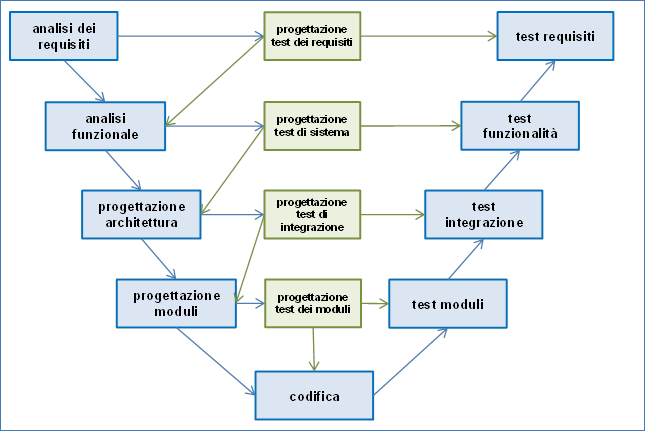
\includegraphics[width=15cm, height=10cm]{./documenti/modello_a_v.png}
    \caption{Figura 0: Modello a V}
\end{figure}


\subsection{Test di Unità}
Il \textit{test di unità} sono una tipologia di testing\textsubscript{G} del software in cui singole unità o componenti del software vengono testate in isolamento. Le unità possono essere singole funzioni, procedure, metodi o classi. L'obiettivo del test di unità è verificare che ciascuna unità funzioni correttamente secondo le specifiche e che produca i risultati attesi. Abbiamo deciso che questo tipo di testing sarà in larga parte automatizzato, per ottimizzare i costi e le tempistiche dedicate a questo processo.

\subsection{Test di Integrazione}
I \textit{test di integrazione} sono una fase del processo di testing\textsubscript{G} in cui le diverse unità o del software vengono combinate e testate insieme come gruppo. L'obiettivo principale è verificare che le singole unità, testate precedentemente in modo isolato tramite i test di unità, funzionino correttamente quando integrate e collegate tra loro. Durante i test di integrazione, vengono identificati e risolti eventuali problemi di interfacciamento tra le diverse unità e vengono verificate le interazioni tra di esse. L'obiettivo finale è garantire che l'intero sistema funzioni come previsto e che tutte le interazioni tra le sue parti siano corrette.

\subsection{Test di Sistema}
I \textit{test di sistema} sono una fase del processo che si concentra sull'analisi e la verifica del sistema nel suo complesso rispetto ai requisiti specificati. L'obiettivo principale è garantire che il sistema soddisfi tutte le funzionalità e i requisiti richiesti dal cliente o specificati nel documento di specifica dei requisiti. Durante i test di sistema, vengono eseguiti scenari di test realistici per simulare l'utilizzo del software in un ambiente di produzione. I risultati dei test di sistema sono utilizzati per valutare se il sistema è pronto per il rilascio o se sono necessari ulteriori miglioramenti e correzioni.

\begin{center}
    \begin{tabular}{P{5em} P{21em} P{6em} P{6em}}
    \rowcolor{Blue}
    \custombold{ID Test\textsubscript{G}} & \custombold{Descrizione} & \custombold{ID Requisiti} & \custombold{Stato}\\
    \hline
    \rowcolor{LighterBlue}
    TS1 & Verificare che sia possibile accedere alla web-app\textsubscript{G} tramite email e password & ROF1 & NI\\
    \hline
    \rowcolor{LightBlue}
    TS2 & Verificare che sia possibile scrivere le richieste di business & ROF2 & NI\\
    \hline
    \rowcolor{LighterBlue}
    TS3 & Verificare che sia possibile inviare le richieste di business all'IA\textsubscript{G} & ROF3 & NI\\
    \hline
    \rowcolor{LightBlue}
    TS4 & Verificare che sia possibile visualizzare l'andamento del progetto dalla web-app\textsubscript{G} & ROF4 & NI\\
    \hline
    \rowcolor{LighterBlue}
    TS5 & Verificare che sia possibile per l'attore\textsubscript{G} Cliente inviare un feedback riguardo l'implementazione di una user story\textsubscript{G} generata & ROF5 & NI\\
    \hline
    \rowcolor{LightBlue}
    TS6 & Verificare che si riceva una notifica una volta che una user story\textsubscript{G} è contrassegnata come completata & RDF6 & NI\\
    \hline
    \rowcolor{LighterBlue}
    TS7 & Verificare che sia possibile il tag\textsubscript{G} del codice utilizzando il plug-in\textsubscript{G} & ROF7 & NI\\
    \hline
    \rowcolor{LightBlue}
    TS8 & Verificare che sia possibile per l'attore\textsubscript{G} Sviluppatore il poter vedere la lista di user/epic stories\textsubscript{G} che gli sono state assegnate & ROF8 & NI\\
    \hline
    \rowcolor{LighterBlue}
    TS9 & Verificare che quando viene assegnata una epic/user story\textsubscript{G} l'attore Sviluppatore venga notificato tramite la web-app\textsubscript{G} & RDF9 & NI\\
    \hline
    \rowcolor{LightBlue}
    TS10 & Verificare che sia possibile inviare il codice all'IA\textsubscript{G} per la verifica & ROF10 & NI\\
    \hline
    \end{tabular}
\end{center}
\begin{center}
    \begin{tabular}{P{5em} P{21em} P{6em} P{6em}}
    \rowcolor{Blue}
    \custombold{ID Test\textsubscript{G}} & \custombold{Descrizione} & \custombold{ID Requisiti} & \custombold{Stato}\\
    \hline
    \rowcolor{LighterBlue}
    TS11 & Verificare che sia possibile visualizzare le epic/user stories\textsubscript{G} generate & ROF11 & NI\\
    \hline
    \rowcolor{LightBlue}
    TS12 & Verificare che sia possibile per l'attore Project Manager\textsubscript{G} l'invio di feedback riguardante le epic/user stories generate dall'IA\textsubscript{G} & ROF12 & NI\\
    \hline
    \rowcolor{LighterBlue}
    TS13 & Verificare che sia possibile per l'attore Project Manager richiedere la divisione delle user stories valutate come troppo grandi & ROF13 & NI\\
    \hline
    \rowcolor{LightBlue}
    TS14 & Verificare che sia possibile per l'attore Project Manager assegnare le epic/user stories a gli attori Sviluppatore & ROF14 & NI\\
    \hline
    \rowcolor{LighterBlue}
    TS15 & Verificare che venga inviata una notifica all'attore Project Manager quando vengono generate le epic/user stories & RDF15 & NI\\
    \hline
    \rowcolor{LightBlue}
    TS16 & Verificare che sia possibile per l'attore Project Manager richiedere la modifica di epic/user stories all'IA & ROF16 & NI\\
    \hline
    \rowcolor{LighterBlue}
    TS17 & Verificare che sia possibile per l'attore Sviluppatore visualizzare l'andamento delle epic/user stories assegnate & ROF17 & NI\\
    \hline
    \rowcolor{LightBlue}
    TS18 & Verificare che il plug-in\textsubscript{G} supporti i linguaggi Typescript\textsubscript{G} e Javascript\textsubscript{G} & ROF20 & NI\\
    \hline
    \rowcolor{LighterBlue}
    TS19 & Verificare che il plug-in supporti i linguaggi Kotlin\textsubscript{G} e Swift\textsubscript{G} & RDF21 & NI\\
    \hline
    \end{tabular}
    \captionof{table}{Tabella dei test di sistema}
\label{tab:testSistema}
\end{center}

\subsection{Test di Accettazione}
I \textit{test di accettazione} sono una fase finale in cui il sistema viene valutato dal cliente per determinare se soddisfa i requisiti concordati e se è pronto per il rilascio. Questi test sono orientati a verificare che il sistema sia conforme alle aspettative e alle necessità degli utenti e che sia in grado di svolgere le funzioni previste in modo efficace ed efficiente. L'obiettivo principale è confermare che il software sia pronto per essere messo in produzione e che risponda alle aspettative del cliente. I risultati dei test di accettazione sono fondamentali per prendere decisioni riguardanti il rilascio del prodotto e possono influenzare eventuali modifiche o miglioramenti futuri.

\subsection{Test di Regressione}
I \textit{test di regressione} mirano a verificare che le modifiche apportate al codice sorgente o al sistema non abbiano introdotto nuovi difetti o rotto funzionalità esistenti. Questi test vengono eseguiti dopo ogni modifica al software, come aggiornamenti, correzioni di bug o nuove implementazioni. L'obiettivo è assicurarsi che le modifiche non abbiano impatti indesiderati sul comportamento del sistema, specialmente su funzionalità precedentemente testate e funzionanti correttamente. L'obiettivo del gruppo è raggiungere la massima automazione possibile dei test di regressione, al fine di ridurre i tempi di esecuzione e garantire una copertura completa dei test.


\section{Resoconto attività di verifica}
\subsection{Verifica documenti}
\subsubsection{Indice di Gulpease}

    \begin{figure}[H]
    \centering
    \includegraphics{documenti/grafici/indice_di_Gulpease.png}
     \caption{Figura 1: indice di Gulpease per periodo}
    \end{figure}

    L'andamento discendente dell'Indice di Gulpease nei documenti analizzati suggerisce una tendenza verso una maggiore complessità e articolazione del linguaggio nel corso del tempo. Questo declino potrebbe riflettere cambiamenti nella struttura dei testi o nell'approccio alla scrittura, sottolineando l'importanza di un'attenta valutazione delle competenze linguistiche e comunicative nel contesto attuale.



\subsubsection{Errori ortografici}
   \begin{figure}[H]
    \centering
    \includegraphics{documenti/grafici/errori_ortografici.png}
     \caption{Figura 2: errori ortografici per periodo}
    \end{figure}
     Il progressivo e costante ridursi del numero di errori ortografici nei documenti analizzati dimostra un notevole miglioramento della qualità della scrittura nel tempo. Questo risultato evidenzia l'efficacia di misure correttive e di una maggiore attenzione alla precisione nell'uso della lingua.
\subsection{Verifica processi}
\subsubsection{Stima al completamento}
\begin{figure}[H]
    \centering
    \includegraphics{documenti/grafici/costo_effettvo_e_stima_al_completamento.png}
    \caption{Figura 3: Revisione del valore stimato per la realizzazione del progetto}
    \end{figure}
    L'analisi del costo effettivo e della stima al completamento del progetto indica un utilizzo attuale di circa 8000€, con un saldo residuo di circa 4000€ per raggiungere il completamento totale. Questo risultato evidenzia una gestione finanziaria attenta e prudente, mantenendo il progetto all'interno dei limiti del budget previsto. Tuttavia, è importante rimanere vigili e continuare a monitorare da vicino le spese rimanenti per garantire che il progetto sia completato in modo efficiente e senza sorprese finanziarie.
\subsubsection{Valore guadagnato \& valore previsto}
\begin{figure}[H]
    \centering
    \includegraphics{documenti/grafici/valore_guadagnato_e_previsto.png}
    \caption{Figura 4: Valore delle attività realizzate e costo pianificato per realizzare le rimanenti}
    \end{figure}
    L'analisi del valore guadagnato e del valore previsto evidenzia una stretta correlazione tra le previsioni progettuali e i risultati effettivamente ottenuti, come indicato dalla quasi costante equivalenza tra i due valori nel corso del tempo. Sebbene si sia verificato un breve periodo in cui il valore guadagnato è risultato inferiore alle aspettative, è importante notare che il progetto è stato in grado di recuperare e allinearsi nuovamente con le previsioni nel periodo successivo.
\subsubsection{Costo e stima al completamento}
    
    \begin{figure}[H]
    \centering
    \includegraphics{documenti/grafici/costo_e_stima.png}
    \caption{Figura 5: Costo effettivamente sostenuto e valore stimato per la realizzazione delle rimanenti attività}
\end{figure}
L'analisi del costo e della stima al completamento al periodo attuale rivela un leggero scostamento tra il budget utilizzato e quello previsto per il progetto. Mentre il budget utilizzato risulta essere leggermente più alto delle previsioni in questo punto temporale, è essenziale considerare attentamente le ragioni dietro questo scostamento e prendere le misure necessarie per mitigare eventuali ulteriori variazioni.

\subsubsection{Variazione programmazione \& variazione costi}
\begin{figure}[H]
    \centering
    \includegraphics{documenti/grafici/variazione_programmazione_e_costi.png}
    \caption{Figura 6: Variazione programmazione e variazione costo per periodo}
    \end{figure}
    L'analisi della variazione tra la programmazione e i costi indica che la Cost Variance è leggermente superiore alla Schedule Variance. Questo suggerisce che, sebbene il progetto sia rimasto in linea con il programma stabilito, i costi effettivi sono stati maggiori rispetto alle previsioni. Questa discrepanza sottolinea l'importanza di una gestione finanziaria più rigorosa e di un controllo più stretto sui costi nel futuro.
\subsubsection{Stabilità indice dei requisiti}
\begin{figure}[H]
    \centering
    \includegraphics{documenti/grafici/RSI.png}
    \caption{Figura 7: Variazione del numero di requisiti}
    \end{figure}
    L'analisi dell'Indice di Stabilità dei Requisiti (RSI) rivela un trend in aumento nel corso del tempo. Questo aumento progressivo dell'RSI indica una maggiore stabilità dei requisiti del progetto nel tempo. Tale tendenza positiva suggerisce una migliore comprensione e definizione dei requisiti, riducendo la probabilità di cambiamenti o aggiunte significative durante l'implementazione del progetto.
\subsubsection{Attualizzazione rischi}
\begin{figure}[H]
    \centering
    \includegraphics{documenti/grafici/attualizzazione_dei_rischi.png}
    \caption{Figura 8: Rischi verificati per periodo}
    \end{figure}
    L'analisi dell'attualizzazione dei rischi indica un andamento variabile nel corso del tempo. Si osserva un aumento dei rischi verificatisi durante un periodo iniziale, seguito da una successiva diminuzione nel corso del tempo. Questa dinamica potrebbe riflettere l'efficacia delle azioni di mitigazione adottate per gestire i rischi identificati in fase precedente del progetto.
\subsubsection{Metriche di qualità soddisfatte}
\begin{figure}[H]
    \centering
    \includegraphics{documenti/grafici/metriche_soddisfatte.png}
    \caption{Figura 9: Metriche soddisfatte per periodo}
    \end{figure}
    L'analisi delle metriche di qualità soddisfatte evidenzia un trend positivo di miglioramento nel corso del tempo. Si osserva un costante aumento delle metriche soddisfatte, indicando un progressivo miglioramento della qualità nel progetto. Questo risultato può essere attribuito a una maggiore consapevolezza e attenzione alla qualità da parte del team, nonché all'implementazione di processi e pratiche mirate al miglioramento continuo.

\section{Valutazioni per il miglioramento}
In questo paragrafo, esamineremo le sfide incontrate fino alla consegna del progetto e valuteremo le soluzioni adottate dal gruppo. Nella tabella allegata, nella colonna delle soluzioni, sono elencate le strategie che abbiamo identificato per affrontare le sfide riscontrate. È importante sottolineare che il processo di miglioramento è continuo e dinamico, seguendo il principio del ciclo PDCA\textsubscript{G}. Ciò significa che le migliorie vengono implementate in corso d'opera non appena vengono individuate criticità, consentendo al team di adattarsi e migliorare costantemente durante lo sviluppo del progetto.

\subsection{Valutazione sull'organizzazione}
\begin{center}
\begin{tabular}{P{10em} P{13em} P{4em} P{13em}} 
    \rowcolor{Blue}
    \custombold{Criticità} & \custombold{Descrizione} & \custombold{Gravità} &
    \custombold{Soluzione}\\
    \rowcolor{LighterBlue}
     Iniziale carenza di comunicazione con il cliente & Durante le prime fasi di sviluppo abbiamo avuto difficoltà ad ottenere le credenziali per utilizzare gli strumenti da loro richiesti. & Bassa & Abbiamo scelto di focalizzare il lavoro, durante l'attesa, nella redazione dei documenti e aprire un canale di comunicazione più veloce delle mail. Si è scelto Slack per la comunicazione esterna, più rapido e molto utilizzato dall''azienda. è fondamentale sviluppare da parte del team una rapida capacità di reazione.\\ 
    \rowcolor{LightBlue}
     Disparità di impegno tra i membri& Alcuni membri, avendo più impegni accademici o lavorativi, sono stati meno presenti agli incontri o per la realizzazione del progetto. & Media & Ci siamo imegnati nell'autostimare concretamente il tempo che si ha disponibile, comunicando in modo trasparente i nostri impegni settimanali (creando un calendario condiviso su Google Drive) agli altri memebri, e assegnare i compiti quanto più in maniera equa e realistica. \\ 
\end{tabular}
\captionof{table}{Criticità sull'organizzazione}
\label{tab:org}
\end{center}

\subsection{Valutazione sugli strumenti utilizzati}
\begin{center}
\begin{tabular}{P{10em} P{13em} P{4em} P{13em}} 
    \rowcolor{Blue}
    \custombold{Criticità} & \custombold{Descrizione} & \custombold{Gravità} &
    \custombold{Soluzione}\\
    \rowcolor{LighterBlue}
     Complessità nell'integrazione del plug-in\textsubscript{G} & Non avendo mai sviluppato un plug-in è stata difficoltosa la fase di integrazione. & Bassa & Abbiamo scelto di focalizzarci sull'autoapprendimento di tale tecnologia e aggiungere uno Sviluppatore a discapito di altri ruoli più marginali in quella fase. \\ 
    \rowcolor{LightBlue}
     Repository\textsubscript{G} & Difficoltà nel mantenimento dell'ordine, della linea temporale e della versioni\textsubscript{G} dei documenti. & Media & Abbiamo focalizzato una delle fasi di verifica del Verificatore proprio sul controllo della Repository e di fare delle sedute di formazione interna per chi avesse difficoltà nell'uso delle funzionalità più utilizzate dello strumento. \\ 
     \rowcolor{LighterBlue}
     Amazon AWS\textsubscript{G}  & Le librerie di Amazon AWS oltre ad essere moltissime, hanno tutte un prezzo diverso. & Alta & Abbiamo fissato un incontro di formazione da parte del proponente per scegliere in maniera mirata le librerie, in modo tale da essere conformi alle esigenze di costo e non perderci nella fase di analisi, studio dello strumento e scelta delle librerie. Ciò ha ottimizzato a livello di tempistica potenzialmente molto critica per un team inesperto. 
\end{tabular}
\captionof{table}{Criticità negli strumenti utilizzati}
\label{tab:strum}
\end{center}

\subsection{Valutazione sui ruoli}
\begin{center}
\begin{tabular}{P{10em} P{13em} P{4em} P{13em}} 
    \rowcolor{Blue}
    \custombold{Criticità} & \custombold{Descrizione} & \custombold{Gravità} &
    \custombold{Soluzione}\\
    \rowcolor{LighterBlue}
    Verifica superficiale da parte del verificatore.& Alcuni errori sono sfuggiti durante la fase di verifica a causa di una valutazione superficiale. & Media  & Abbiamo implementato checklist di verifica più dettagliate e stringenti.\\ 
    \rowcolor{LightBlue}
     Sviluppatori non allineati agli standard di codifica. & Non sempre il codice è stato conforme agli standard richiesti.&  Media &  Abbiamo svolto sessioni di formazione sui codici di stile e revisione del codice condiviso. Abbiamo condiviso tra membri del team materiale presente sul web fruibile e adatto allo studio individuale. \\ 
     \rowcolor{LighterBlue}
     Inesperienza dell'analista. & Gli analisti, non avendo mai lavorato a un progetto di tale portata, hanno fatto fatica inizialmente ad individuare tutti i requisiti necessari dalle prime sedute. & Media & Abbiamo svolto sessioni  di brainstorming interne e con i proponenti, oltre che col Prof Cardin. \\
    \rowcolor{LightBlue}
    Pianificazione poco realistica da parte del Responsabile. & Data l'inesperienza nell'ambito, la pianificazione e le aspettative sul carico di lavoro non sono state conformi alla realtà.& Bassa & Abbiamo definito sprint più frequenti della media, di due settimane, per mantenere sempre alta la produttività e favorire l'interazione tra i membri del team.
     
\end{tabular}
\captionof{table}{Criticità dei ruoli}
\label{tab:ruoli}

\end{center}

Questo approccio consente una valutazione delle sfide affrontate e delle relative soluzioni, fornendo una base più solida per il miglioramento continuo durante lo sviluppo del progetto.


\end{document}
